\section*{Model Overview}


In order to solve those problems, we will proceed as follows:

\begin{itemize}
    \begin{figure}[htbp]
        \centering
        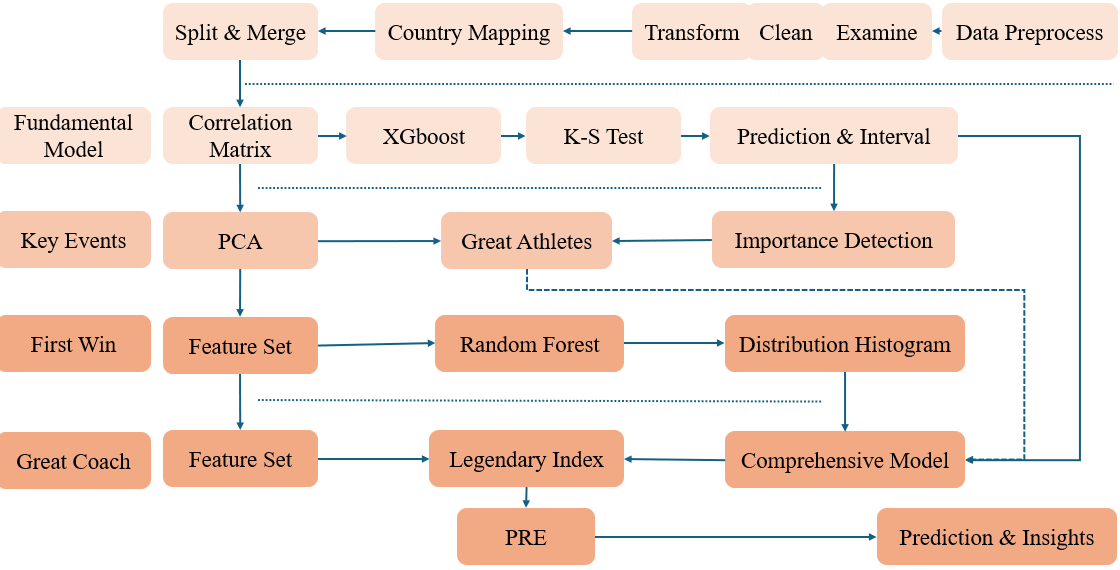
\includegraphics[width=0.8\textwidth]{./figures/figure1_work_flow.png}
        \caption{Flow chart of our work}
        \label{fig:example}
    \end{figure}
    
\item {\bf Presenting our model}. In order to investigate the problem deeper, we divide our task into four models: \textbf{Predicting the Medal of the 2028 LA Olympics}, \textbf{Predicting First Medal Countries}, \textbf{Great Coach Effect}, \textbf{Key Events and Great Athletes}.

\item {\bf Data Processing}.First, We examine, clean and transform the data given and merge them. Then the data is put into the Correlation Coefficient Matrix for further machine learning.

\item {\bf First Medal Model}.Next, We use \textbf{Random Forest} to train the model, giving prediciton of first medal countries.

\item{\bf Performance Analysis}.Then, we calculate the performance of Athletes and countries (on certain sports/events), forming the \textbf{Key Event Model} and the \textbf{Great Coach Model}.

\item {\bf Machine Learning}. Finally, we use \textbf{KS Test} to ensure the precision of the final model.
\end{itemize}
